\documentclass{beamer}
\usepackage{tikz-uml}


\title{TREAT}
\subtitle{Timed Regular Expression to Automaton Transformation}
\author{Group 30}
\institute{Aalborg Universitet}
\date{2024}

\usetheme{Frankfurt}
\useinnertheme{rectangles}

\begin{document}


\frame{\titlepage}

\begin{frame}{Agenda}
    \tableofcontents
\end{frame}

\section{Introduction} % each section gets own category on top bar, each frame within gets a subcategory

%Marcus Section

\begin{frame}{Introduction}
    \centering
    \LARGE\textbf{TREAT} \\
    \vspace{0.5cm}
    \Large\textit{Timed Regular Expression to Automaton Transformation}
\end{frame}

\section{Process}

\begin{frame}{Process}
    \begin{itemize}
        \item Initial Problem
        \item Pivot
        \item Human Readability and Usability
    \end{itemize}
\end{frame}

\begin{frame}{Process}
    \textbf{Initial Problem}

    ``Better Timed Pattern Searching in Log Files''
    \newline
    \begin{itemize}
        \item The paper: ``Timed Regular Expressions''
        \item What should the program contain?
        \begin{itemize}
            \item Parse TREs
            \item Convert TREs to timed automata
            \item Perform checking (Output to UPPAAL)
        \end{itemize}
    \end{itemize}

    Can we output to UPPAAL in a better way?
\end{frame}

\begin{frame}{Process}
    \textbf{Pivot}

    We will still have the same features, but checking will take a lower priority.
    \newline
    \begin{itemize}
        \item Pruning
        \item Graphing
    \end{itemize}
\end{frame}

\begin{frame}{Process}
    \textbf{Human Readability and Usability}

    Focus on efficient transformation from TRE to TA.
    \newline
    \begin{itemize}
        \item TRE input improvement
        \begin{itemize}
            \item Multi-character symbols
        \end{itemize}
        \item CLI
        \item TikZ
    \end{itemize}

    These could have been done regardless, but became a larger focus now.
\end{frame}

\section{Implementation}

\begin{frame}{Implementation}
    %\scalebox{0.9}{
    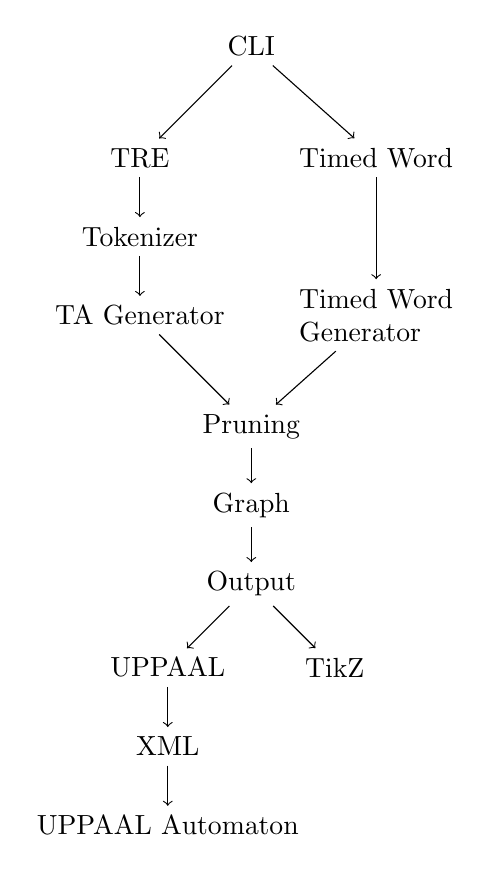
\begin{tikzpicture}[node distance = 1cm, auto]\label{fig:TREATdiagram}
        \node (CLI) {CLI};
        
        \node (TRE) [node distance = 2cm, below left of = CLI] {TRE};
        \node (TimedWord) [node distance = 3cm, right of = TRE] {Timed Word};
        \node (Tokenizer) [below of = TRE] {Tokenizer};
        \node (TAGenerator) [below of = Tokenizer] {TA Generator};
        \node (Pruning) [node distance = 2cm, below right of = TAGenerator] {Pruning};
        \node (Graph) [below of = Pruning] {Graph};
        \node (Output) [below of = Graph] {Output};
        \node (UPPAAL) [node distance = 1.5cm, below left of = Output] {UPPAAL};
        \node (XML) [below of = UPPAAL] {XML};
        \node (UPPAALAutomaton) [below of = XML] {UPPAAL Automaton};
        \node (TikZ) [node distance = 1.5cm, below right of = Output] {TikZ};
        \node (TimedWordGenerator) [node distance = 3cm, right of = TAGenerator,  align=left] {Timed Word\\Generator};
    
        \draw[->] (CLI) -- (TRE);
        \draw[->] (TRE) -- (Tokenizer);
        \draw[->] (Tokenizer) -- (TAGenerator);
        \draw[->] (TAGenerator) -- (Pruning);
        \draw[->] (Pruning) -- (Graph);
        \draw[->] (Graph) -- (Output);
        \draw[->] (Output) -- (UPPAAL);
        \draw[->] (UPPAAL) -- (XML);
        \draw[->] (XML) -- (UPPAALAutomaton);
        \draw[->] (Output) -- (TikZ);
        \draw[->] (CLI) -- (TimedWord);
        \draw[->] (TimedWord) -- (TimedWordGenerator);
        \draw[->] (TimedWordGenerator) -- (Pruning);
    \end{tikzpicture}
}
  % Doesn't work because no TikZ
\end{frame}

\begin{frame}[shrink=20]{Parser}
    
\textbf{CFG}

TimedRegex := Rename

\qquad	$\mid$ $\epsilon$

Rename := Intersection renameStart RenameSymbols renameEnd

\qquad $\mid$ Intersection

RenameSymbols := match match renameSeparator RenameSymbols

\qquad $\mid$ match match

Intersection := Union intersection Intersection

\qquad $\mid$ Union

Union := Concatenation union Union

\qquad $\mid$ Concatenation

Concatenation := Interval Concatenation

\qquad $\mid$ Interval absorb Concatenation

\qquad $\mid$ Interval

Concatenation := Concatenation Interval

\qquad $\mid$ Interval

Interval := Unary IntervalStartEnd Number intervalSeperator Number IntervalStartEnd

\qquad $\mid$ Unary

IntervalStartEnd := intervalOpen

\qquad $\mid$ intervalClose

Number := digit Number

\qquad $\mid$ digit

Unary := Match guaranteedIterator

\qquad $\mid$ Match guaranteedIterator absorb

\qquad $\mid$ Match iterator

\qquad $\mid$ Match iterator absorb

\qquad $\mid$ Match

Match := parenthesisStart Rename parenthesisEnd

\qquad $\mid$ match

\qquad $\mid$ matchAny


\end{frame}

\begin{frame}{Parser}
    AST UML goes here
    %\input{}  
\end{frame}

\begin{frame}{TA UML}
    \begin{tikzpicture}
    \umlclass{TA}{clockCount: int\\edges/locations}{}
    
    \umlclass[x=-4, y=-4]{Location}{id: int\\initial: bool\\}{}
    \umlcompo[geometry=|-|,attr1=0..*|,attr2=1|,pos1=1.8,pos2=0.2]{TA}{Location}
    
    \umlclass[y=-4]{Edge}{id: int\\ranges\\resetClocks}{}
    \umlcompo[geometry=|-|,attr1=|0..*,attr2=1|,pos1=1.8,pos2=0.2]{TA}{Edge}
    \umlassoc{Edge}{Location}

    \umlclass[x=4,y=-4]{Clock}{id: int}{}
    \umlcompo[geometry=|-|,attr1=|0..*,attr2=1|,pos1=1.8,pos2=0.2]{TA}{Edge}
    \umlassoc{Edge}{Clock}
    
\end{tikzpicture}
\end{frame}


%End of Marcus section

\end{document}